%!TEX root = ../TaxationPlan.tex

We now consider how to implement fees in a world where the system margin grows over time
according to a deterministic process. One of the reasons that it is important to model growth in
this system is that, if people believe that there will be higher buybacks in the future, then we
might be able to sustain lower buybacks today.

For simplicity, we assume that margin follows

$$M_{t+1} = M_{t} + g M_{t} \left(1 + \frac{M_{t}}{\bar{M}} \right)$$

This process, known as logistic growth, generates ``S-shaped'' growth. We can see the implications
that this process has for the total system margin in Figure \ref{fig:dg_margin_growth}.

\begin{center}
  \begin{figure}[H]
    \scalebox{0.65}{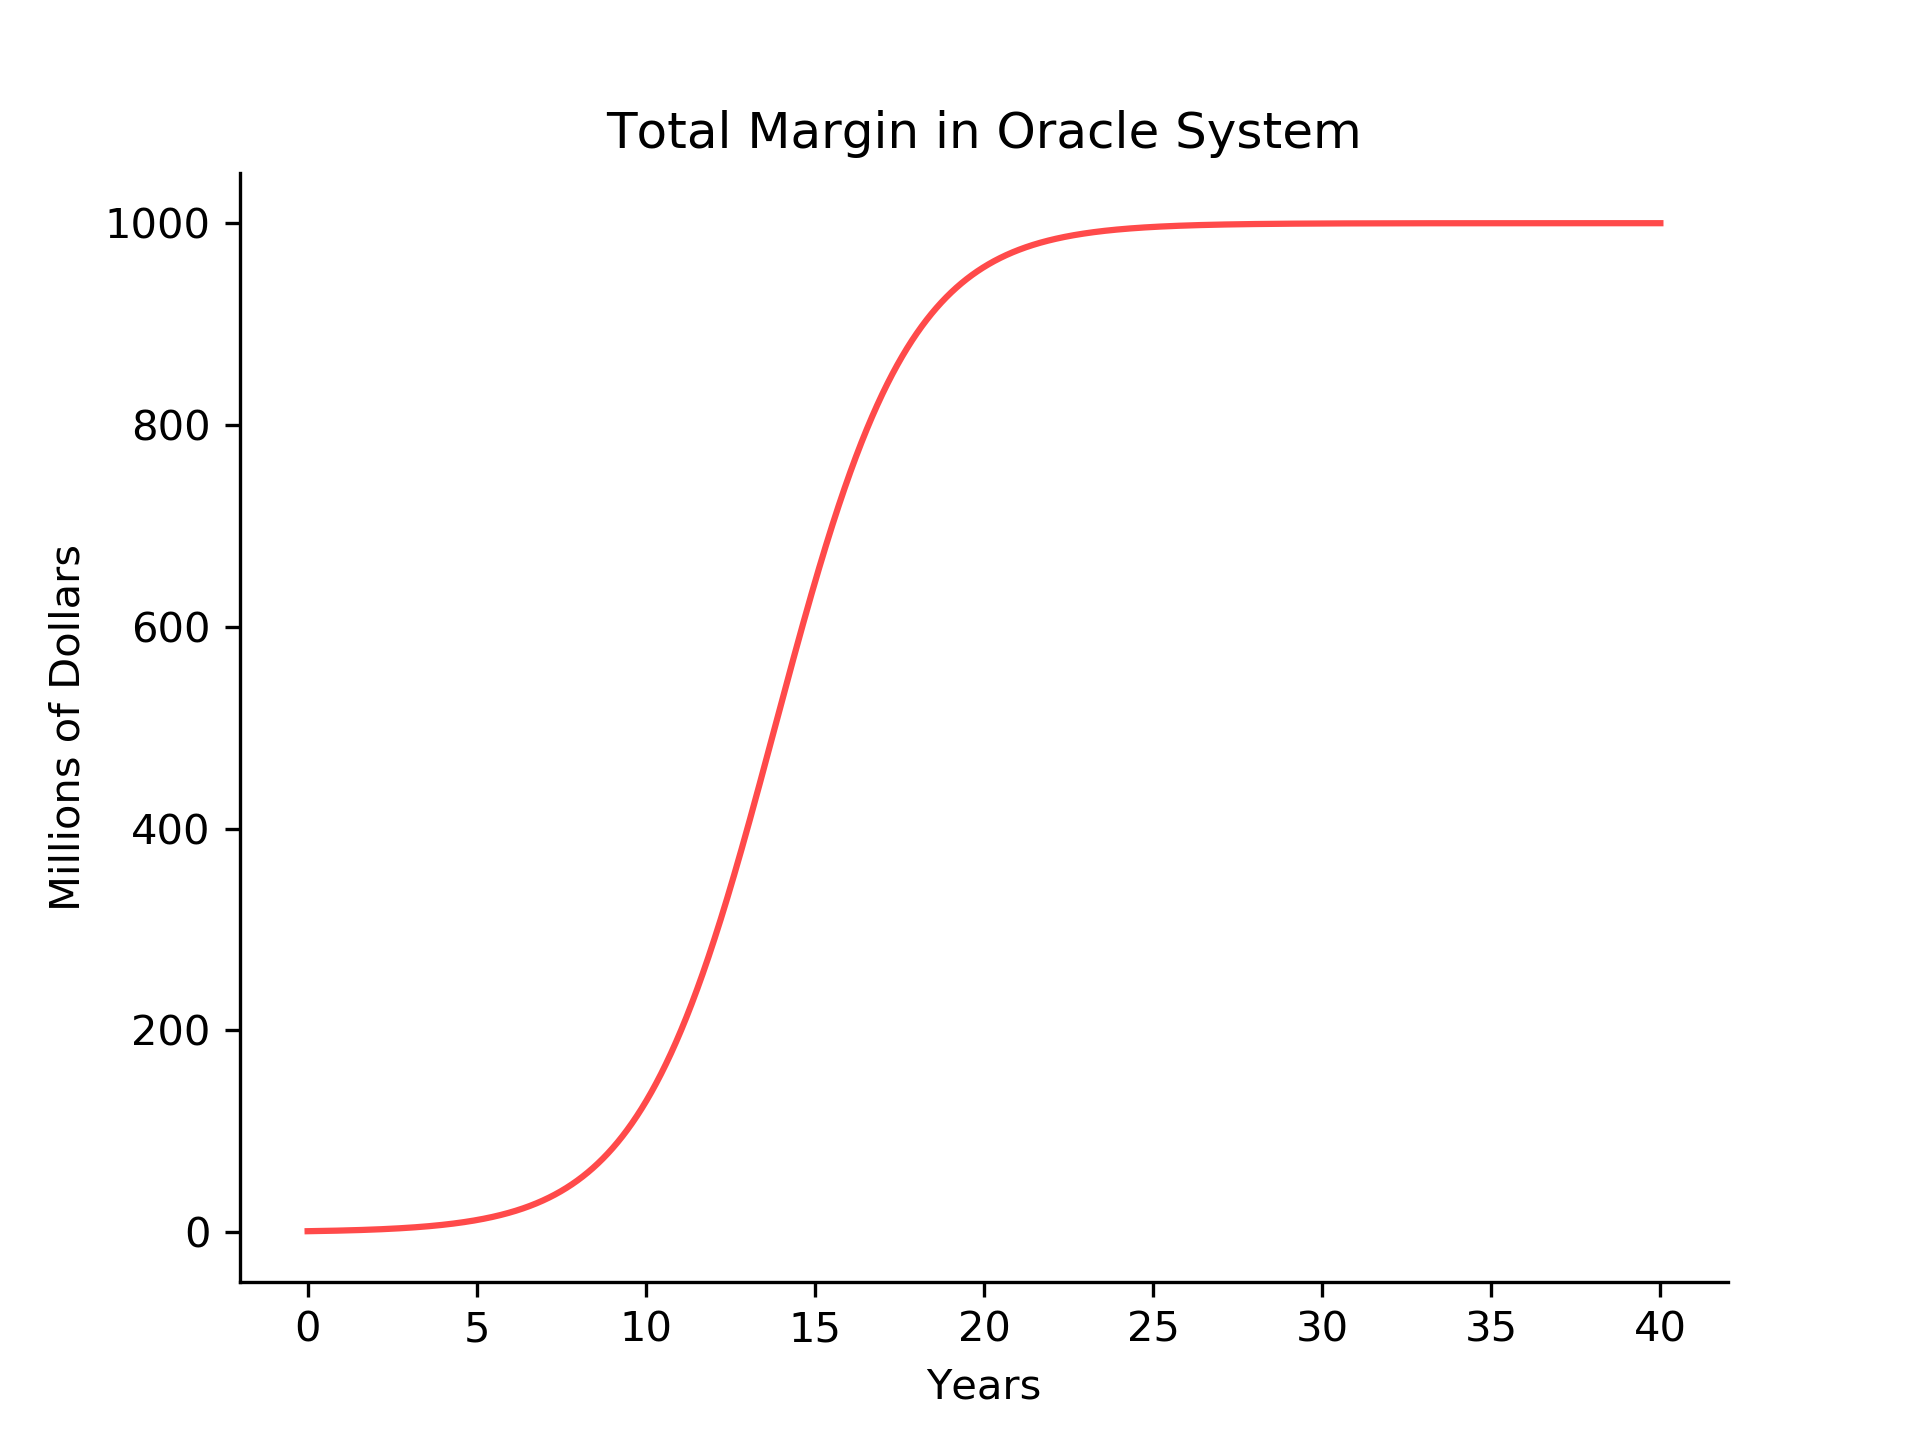
\includegraphics{./TaxationPlanImages/MarginGrowth.png}}
    \label{fig:dg_margin_growth}
  \end{figure}
\end{center}

We assume that we would like to charge the minimum amount of fees while maintaining the system's
incorruptibility. This produces the following mathematical program:

\begin{align*}
  \min_{F_t} \; &E \left[ \sum_{t=0} \left(\frac{1}{1 + r} \right)^t F_t \right] \\
  &\text{subject to} \\
  PfC_t &\leq \frac{1}{2} P_t S_t = \frac{1}{2} E \left[ \sum_{s=0} \left(\frac{1}{1 + r}\right)^s  X_{t + s} \right] \\
  X_{t} &= F_t \\
  0 &\leq F_t \\
  F_t &\leq \bar{\tau} \bar{M} \\
  M_{t+1} &= M_{t} + g M_{t} \left(1 + \frac{M_t}{\bar{M}} \right)
\end{align*}

We can solve this program indirectly by choosing an $s$ such that $M_s \approx \bar{M}$. At this
point, we have arrived in the steady state and the fee rate implemented will be
$F_t = \bar{\tau} M_t$. We can then step back by one period to $t = s - 1$ and compute what the
required $X_t$ in that period would be. We can proceed to step this back until we reach our initial
condition of $M_0$ which traces out a path of fee collections. This process generates a sequence of
fees that look like Figure \ref{fig:dg_tax_growth}.

\begin{center}
  \begin{figure}[H]
    \scalebox{0.65}{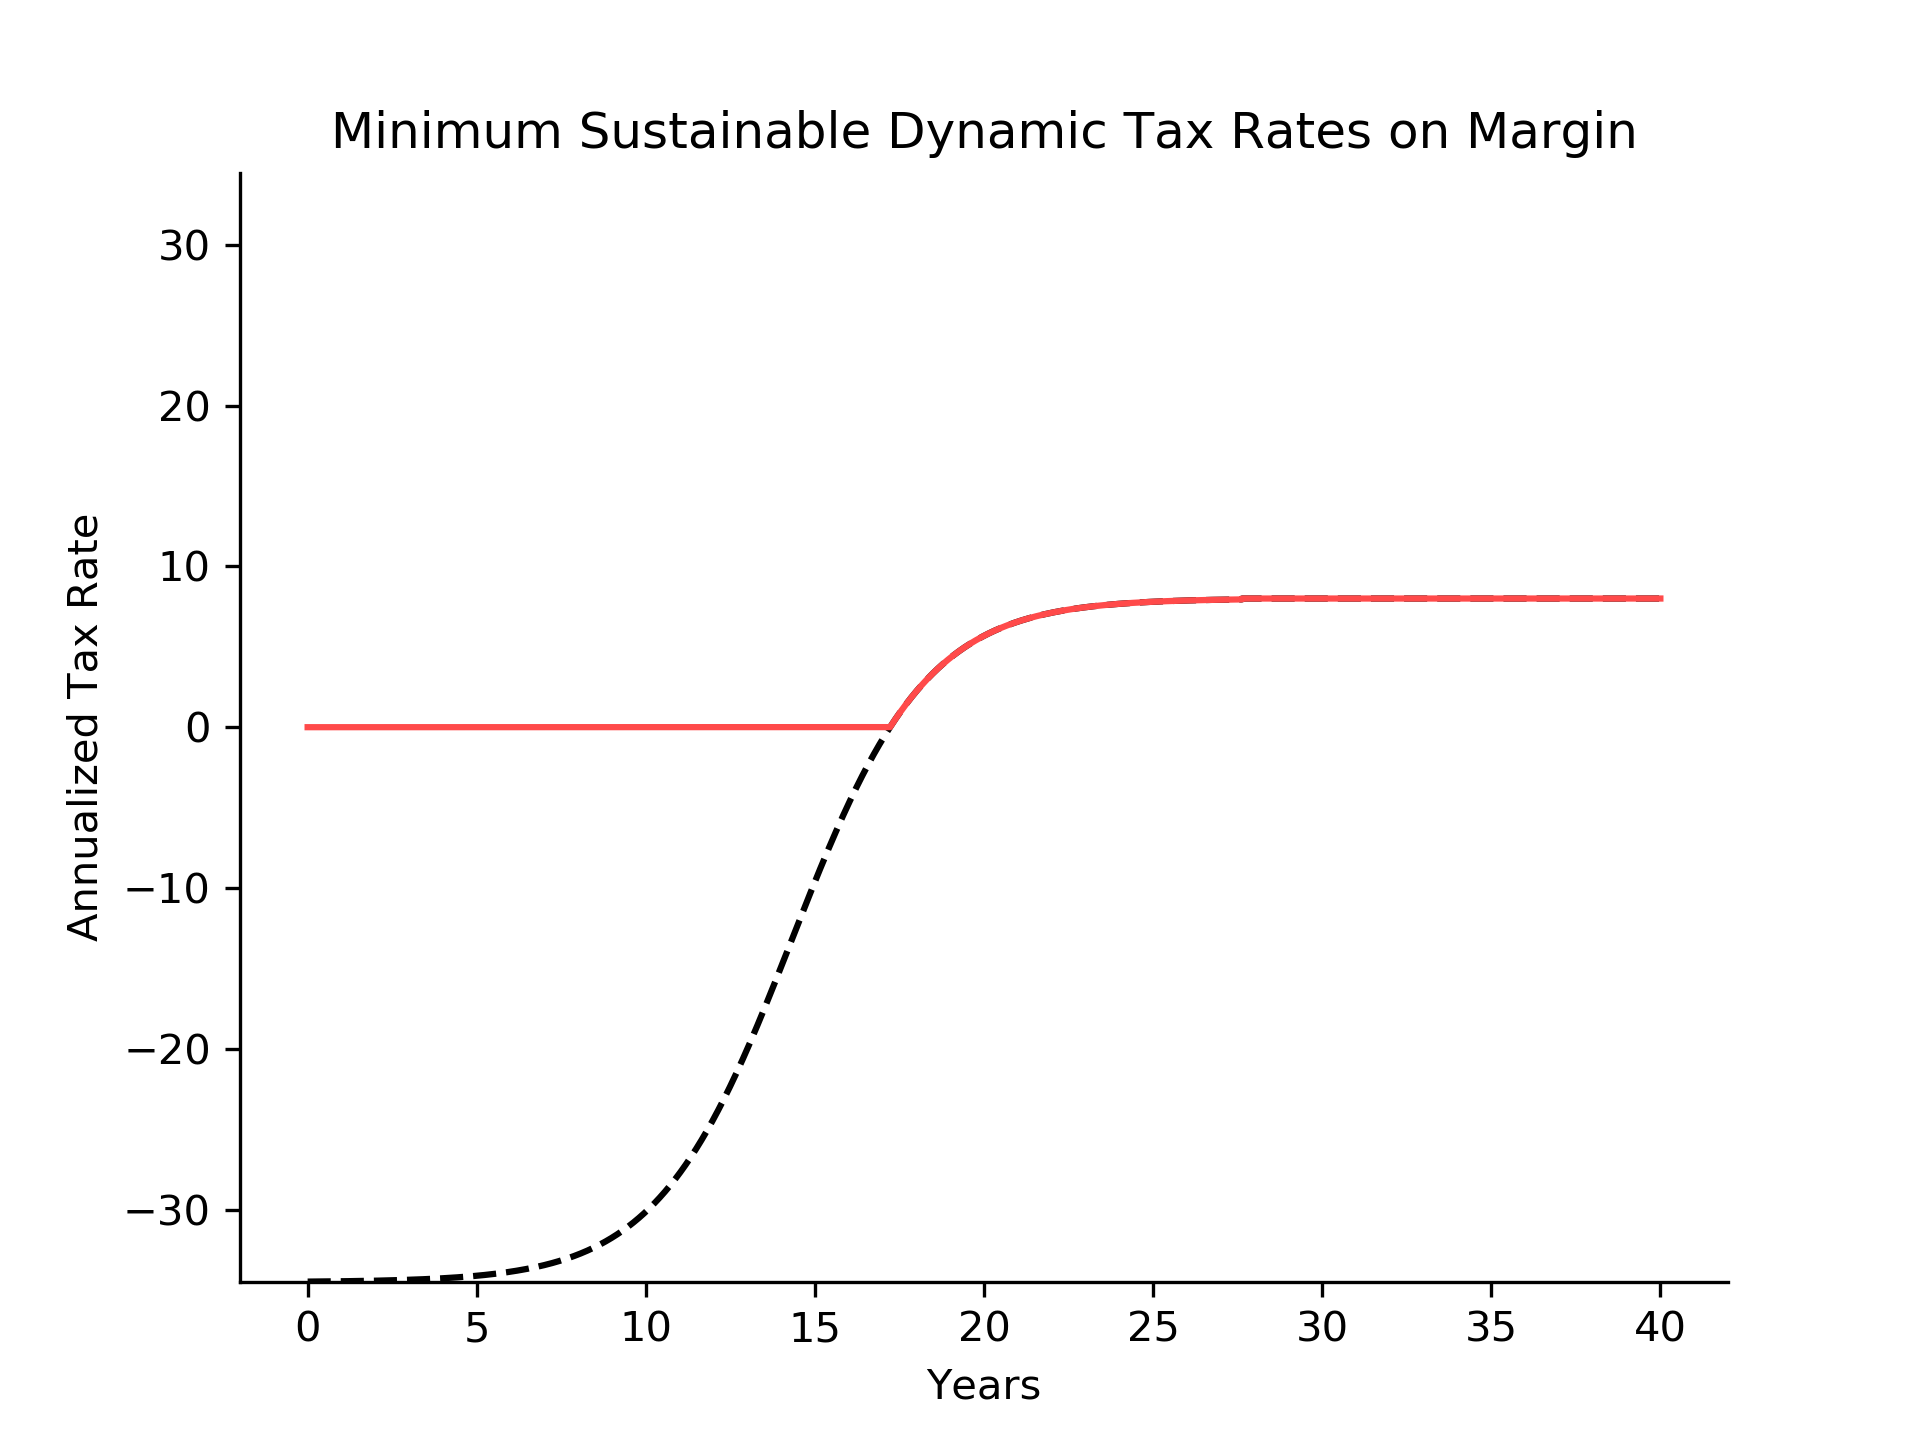
\includegraphics{./TaxationPlanImages/TaxRates.png}}
    \label{fig:dg_tax_growth}
  \end{figure}
\end{center}

We plot the solution to two different mathematical programs. The first, plotted as a solid line,
corresponds to the program that we described above. The second, plotted as a dashed line,
corresponds to what fee rates would be if we did not impose the non-negativity constraint. Notice
that in the case in which there is no non-negativity constraint, the fees go negative in order to
meet the $PfC < CoC$ constraint with equality.

The most interesting observation we make from this chart is that fees can start low and stay low
for a prolonged period of time before rising to the steady state levels. The reason that this
satisfies the $PfC < CoC$ inequality is that individuals understand that there will be growth in
the system --- The future promise of increased buybacks in the future is enough to secure the system
while it is new (and small).

We can be see this by looking at the equation that determines the $CoC$:

\begin{align*}
  CoC_t &= \chi p_t S_t = \chi E \left[ \sum_{s=0}^{\infty} \left(\frac{1}{1 + r} \right)^s X_{t+s} \right]
\end{align*}

High values of $X_{t + s}$ increase the cost of corruption in period $t$. This insight is somewhat
general, but may be potentially too strong in this model due to the fact that there is certainty
about the future growth. This concern motivates our next section in which we introduce uncertainty
about the growth of the system.
